\documentclass[12pt]{article}

\newcommand{\GroupId}{CC09-7}
\newcommand{\assignment}{project-usability}

\NeedsTeXFormat{LaTeX2e}
\usepackage[osf]{mathpazo}
\usepackage[svgnames]{xcolor}
\usepackage[T1]{fontenc}
\usepackage{amsmath,amsthm,amsfonts,amssymb,mathtools}
\usepackage{multicol}
\usepackage{float}
\usepackage[margin=2.7cm,a4paper]{geometry}
\usepackage{tasks}
\usepackage{xstring}
\usepackage[tikz]{mdframed}
\usepackage{environ}
\usepackage{subcaption}
\usepackage{etoolbox}
\usepackage{booktabs}
\usepackage{fourier-orns}
\usepackage{kvoptions}
\usepackage{units}
\usepackage{hyperref}
\usepackage{url}
\geometry{a4paper, margin=1in}
\setlength{\parindent}{2em}
\usepackage{graphicx}
\usepackage{subcaption}

% math config

\DeclarePairedDelimiter\ceil{\lceil}{\rceil}
\DeclarePairedDelimiter\abs{\lvert}{\rvert}
\DeclarePairedDelimiter\set{\{}{\}}

% headers

\usepackage{fancyhdr}
\addtolength{\headheight}{2.5pt}
\pagestyle{fancy}
\fancyhead{} 
\fancyhead[L]{\sc info2222} 
\renewcommand{\headrulewidth}{0.75pt}

% update these headers
\fancyhead[C]{\sc Group Id: \GroupId}
\fancyhead[R]{Assignment \assignment}

\begin{document}

\section{User Investigation}

\subsection{Introduction}

\hspace{2em}In our project, we chose students as the target user group and conducted a survey through Ed and tutorial classes to gain a deeper understanding of their needs and preferences. The students who participated in the survey were mainly from computer science-related departments.

Through the survey, we found that students primarily use WeChat (55.1\%) and Instagram (24.5\%) to communicate with friends (61.2\%) and classmates (28.6\%). They like the user-friendly interface of these chat applications (71.4\%) and prefer the option to set multilingual support (54.5\%). Students hope that chat rooms will allow only the group owner to invite friends (63.3\%). Opinions were divided on whether new users should be able to see chat room history (55\% in favor, 45\% against). Based on these findings and lecture slides \cite{7.users-designs.pptx}, we conducted a PACT analysis for this group of computer science students and constructed relevant personas. The statistics for each question and the complete survey data are provided in the appendix (\ref{survey}).

\subsection{PACT Analysis}
\hspace{2em}\textbf{People:} (98\%) of respondents are students at the University of Sydney, with only one staff member participating. Students primarily use the platform for academic-related activities, such as discussions and posting questions. They also want to communicate with friends. Among the respondents, 55.1\% are currently using WeChat, and 24.5\% are using Instagram, indicating that a design similar to these apps would be more familiar to them. Most respondents are computer science majors, with a few students from other majors.

\textbf{Activities:} The platform's primary use cases include participating in discussions, sharing academic experiences, and asking questions. Additionally, the platform should support students in communicating with friends. In terms of functionality, 61.2\% of users primarily engage in group chats or private chats with friends, and 28.6\% chat with schoolmates. Users prefer that only group owners can invite friends to join group chats (63.3\%) and wish to retain chat history. Both staff and students can post articles and comment on them, with staff having the authority to manage posts and comments. Compared to other features, users highly prefer a friendly interface (71.4\%). Regarding additional features, 54.5\% of users want support for multiple languages.

\textbf{Contexts:} Considering the study and life of university students, they might use the platform both on and off-campus, including at home or during commutes. They can access the site anytime, with peak usage times during the day and evening. Teachers and staff need to be able to access the site at any time to manage student posts, requiring the platform to function reliably across different times and locations, providing a consistent user experience.

\textbf{Technologies:} Considering the usage patterns of university students, the platform must work on various devices, including laptops and phones. Given the diverse usage environments, the platform needs strong adaptive design to ensure a consistent and smooth user experience across all devices.

\subsection{Persona}
\textbf{Name:} Emma Li \\
\textbf{Age:} 20 \\
\textbf{Major:} Computer Science \\
\textbf{Background:} Emma is a second-year computer science student at the University of Sydney. She is proficient in using various technologies and spends a significant amount of time on her laptop and smartphone. She uses chat applications like WeChat and Instagram daily to keep in touch with her friends and classmates. \\
\textbf{Motivations:} 
\begin{itemize}
    \item Share experiences and ask questions related to her studies.
    \item Communicate with friends and classmates for both academic and personal purposes.
    \item Use a platform with a user-friendly interface and multilingual support.
\end{itemize}

\textbf{Frustrations:} 
\begin{itemize}
    \item Difficulty in finding a platform that combines academic and personal communication.
    \item Lack of multilingual support in many existing chat applications.
    \item Confusion caused by complicated interfaces in some chat platforms.
\end{itemize}

\textbf{Preferred Features:} 
\begin{itemize}
    \item User-friendly interface similar to WeChat and Instagram.
    \item Multilingual support.
    \item Ability for group owners to invite friends to join group chats.
    \item Retaining chat history for reference and context.
\end{itemize}

\newpage

\section{Navigation design}

\hspace{2em}We used Optimal Workshop \cite{optimalwork} for card sorting. A total of 11 participants completed the card sorting. The image is shown as figure \ref{cardsorting_overview}. We categorized the multilingual functionality, which we learned about from the previous survey, under the "User settings/profile" card, as this special feature pertains to the entire user interface settings. The similarity matrix of the results is shown in the figure \ref{similarity_matrix}.

\begin{figure}[H]
    \centering
    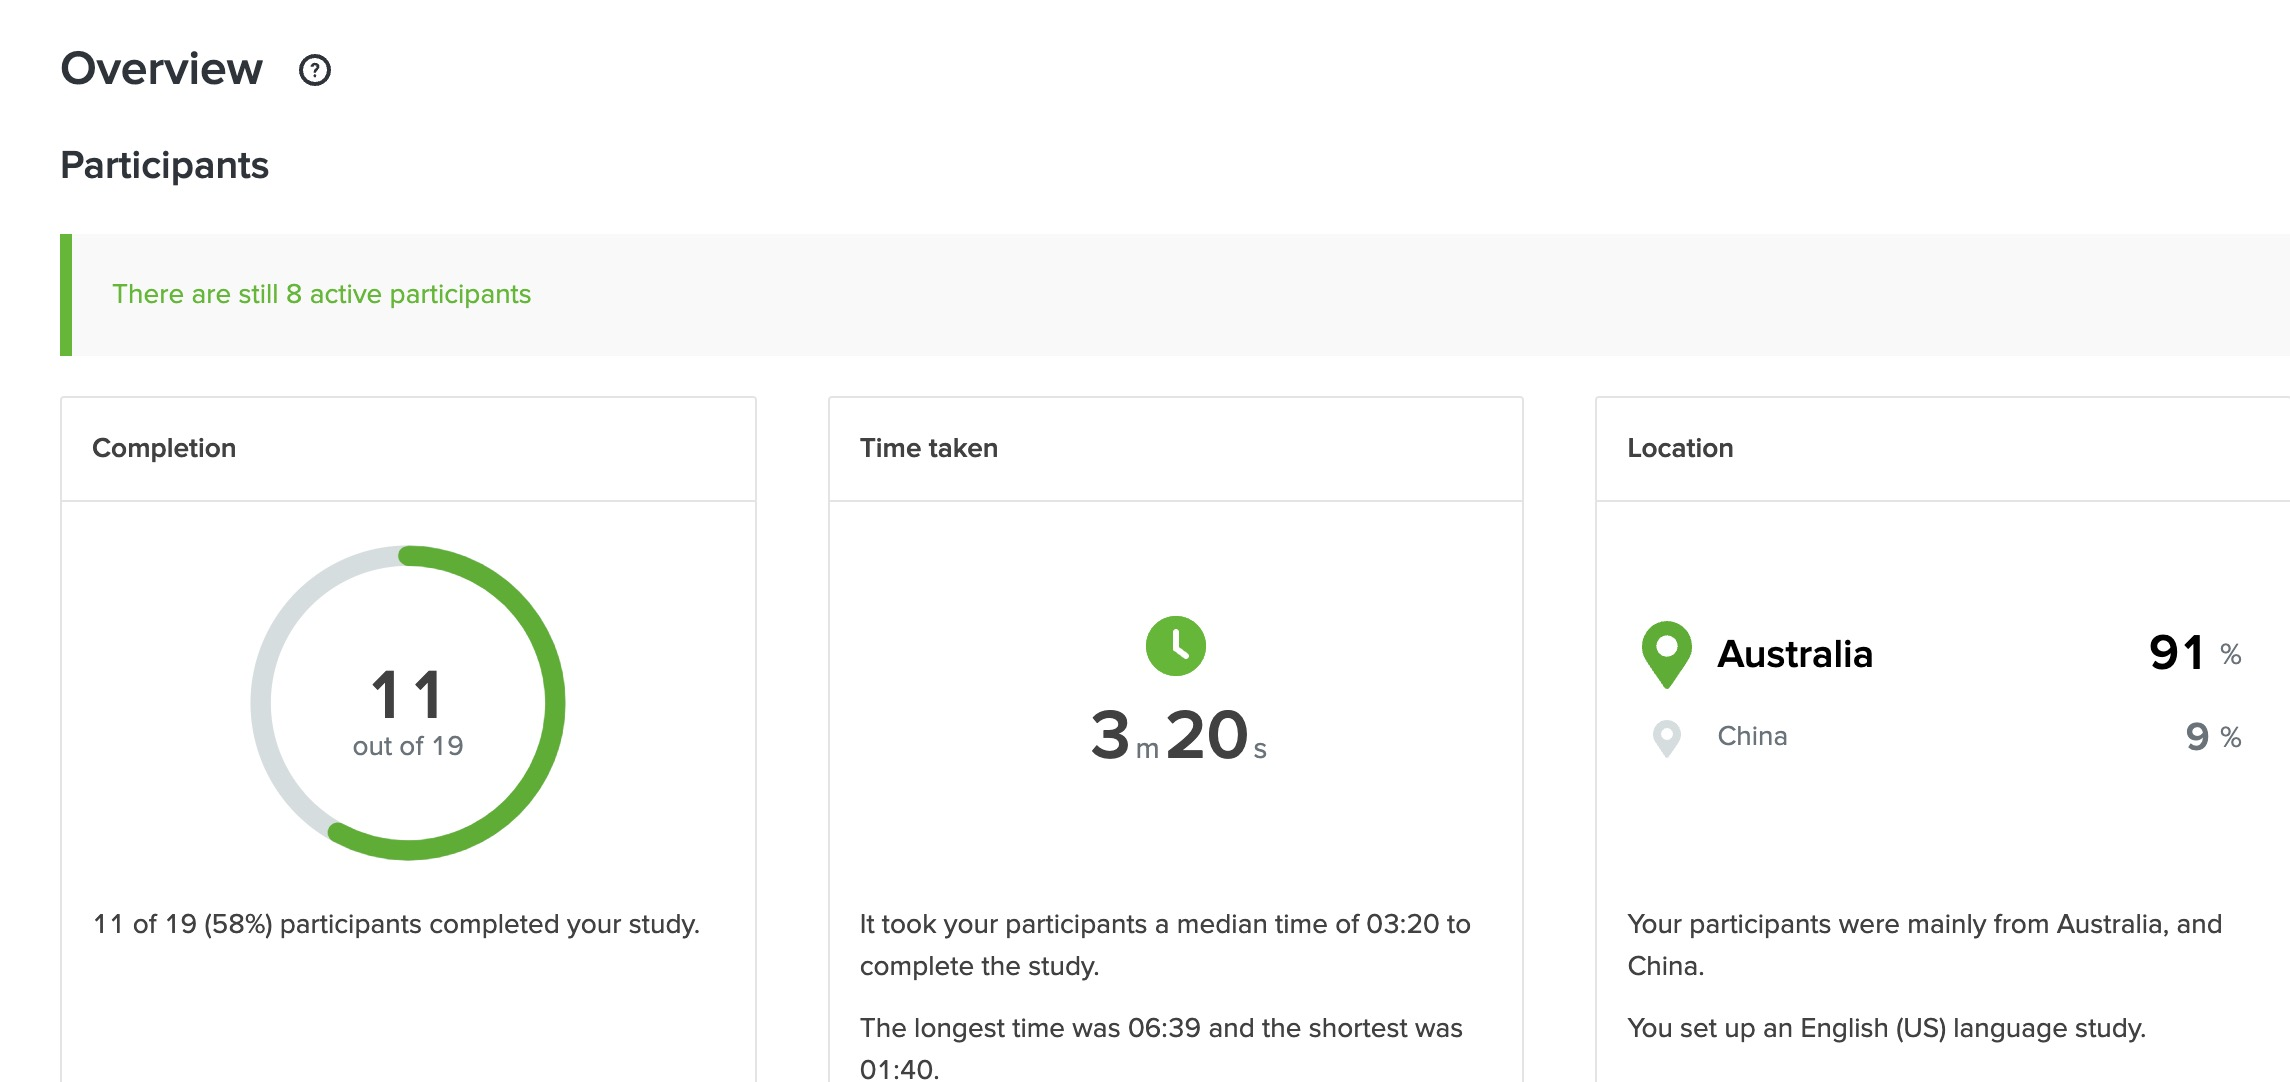
\includegraphics[width=0.9\textwidth]{graphs/cardsorting_overview.jpg}
    \caption{Card Sorting Overview}
    \label{cardsorting_overview}
\end{figure}

\begin{figure}[H]
    \centering
    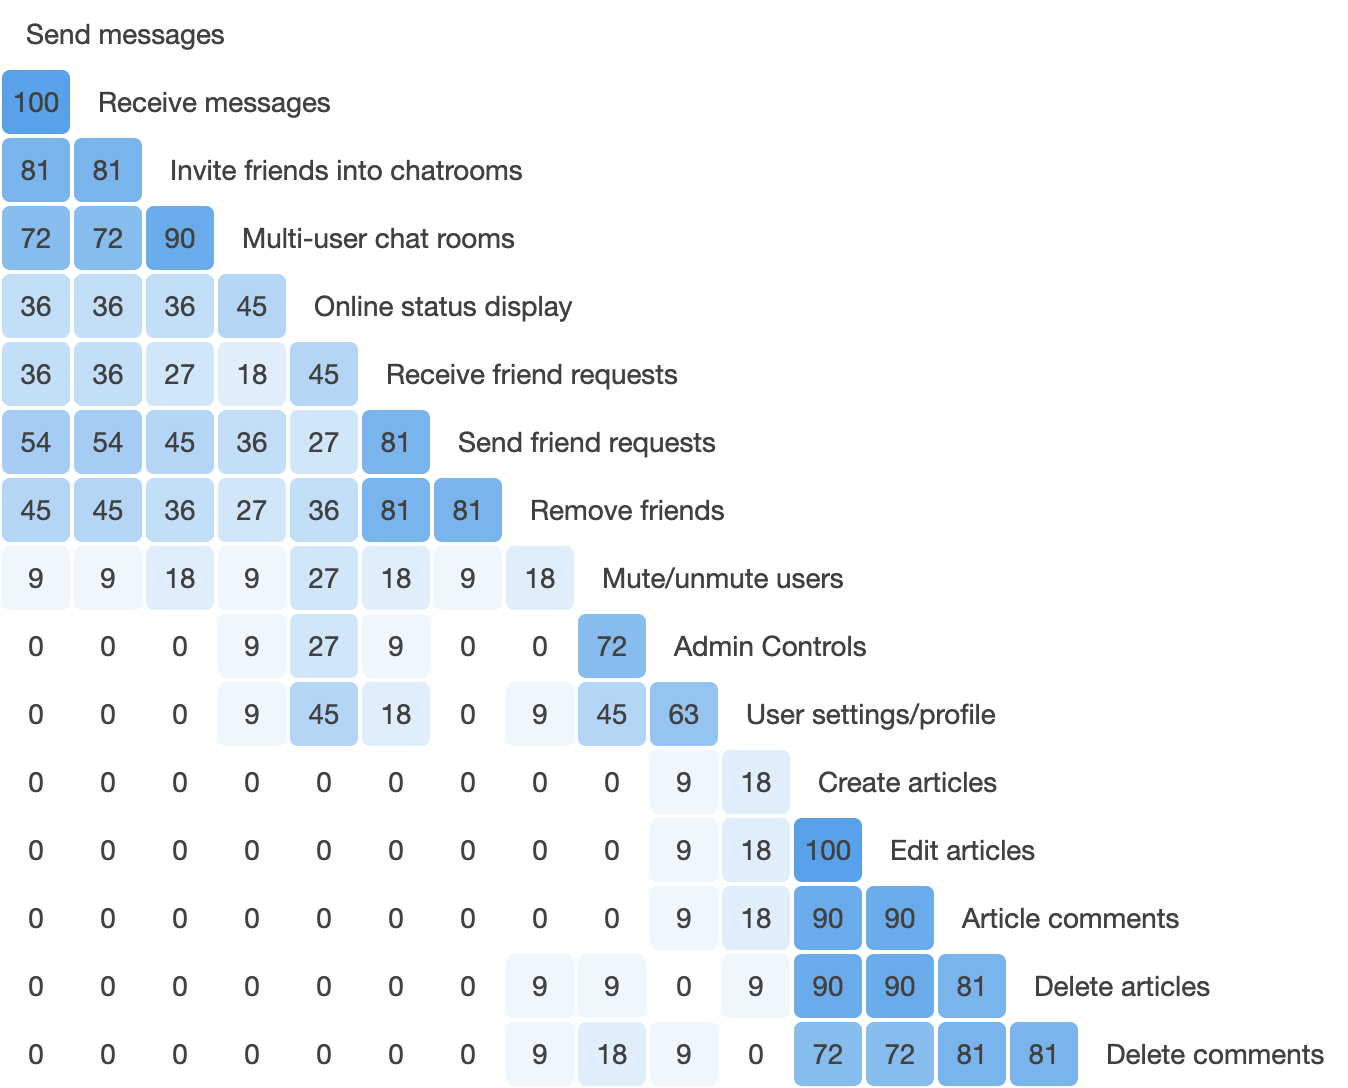
\includegraphics[width=0.8\textwidth]{graphs/Similarity_Matrix.png}
    \caption{Similarity Matrix}
    \label{similarity_matrix}
\end{figure}

\newpage

Based on the similarity matrix, we have categorized as follows:
\begin{multicols}{2}

\subsubsection*{Page: Messages App}
\begin{itemize}
    \item Multi-user chat room
    \item Send message
    \item Receive message
    \item Invite friend into Chatroom
    \item Online status display
    \item Receive friend requests
    \item Send friend request
    \item Remove friend
\end{itemize}

\subsubsection*{Page: Settings}
\begin{itemize}
    \item Admin control
    \item Mute/Unmute User
    \item User settings/profile
\end{itemize}

\columnbreak

\subsubsection*{Page: Knowledge Repo}
\begin{itemize}
    \item Create articles
    \item Delete articles
    \item Edit articles
    \item Article Comments
    \item Delete Articles
    \item Delete Comments
\end{itemize}

\end{multicols}

\section{Design-Evaluate 1}

\subsection{Priority List}

    \hspace{2em}Based on user personas, PACT analysis, and the results of card sorting, we have summarized the following prioritized list of features. Based on the specifications and user needs, we have identified Multi-Person Chat Rooms, Post Publishing, Multi-Language Support, and Enhanced User Interface as primary objectives. These form the core functionalities of the website, with the rest being enhancements built upon these foundational features. The second tier of importance includes supplementary enhancements to the previous functionalities, such as comments under posts and account management capabilities, where staff can manage posts and have the ability to mute and unmute users. Consideration is given to less critical search/filtering functionalities.
    \begin{enumerate}
    \item \textbf{High Priority: Core Features}
        \begin{itemize}
            \item Staff and students can create and delete articles
            \item Staff can delete articles or modify articles made by others
            \item Friends should display whether they are online or not in the friends list
            \item Chatrooms can contain more than 2 users
            \item Users can receive messages from friends even when the recipient is not currently in a chatroom. These messages will be stored in the message history database and loaded when the other user connects to the chatroom
            \item Friends should be able to be removed
            \item Multilingual support - \texttt{User specific function}
            \item User-friendly interface - \texttt{User specific function}
        \end{itemize}

    \item \textbf{Medium Priority: Enhanced User Interaction}
        \begin{itemize}
            \item Students and staff can comment on articles
            \item Staff can delete comments
            \item Different types of staff accounts: academics, administrative staff, and admin users
            \item The role should be displayed in the user’s profile and on any posts they make, viewable to all
            \item Staff can mute/unmute users to prevent them from posting or joining a chatroom
        \end{itemize}

    \item \textbf{Low Priority: Additional Features}
        \begin{itemize}

            \item Provide advanced search and filtering functionalities to help users find articles and information more easily
        \end{itemize}


    \end{enumerate}

\subsection{Low-fidelity Prototype}
    \hspace{2em}Based on the prioritization of features from the previous steps, including card sorting and the website's information architecture, we have designed a low-fidelity prototype consisting of three pages, prioritizing the implementation of core functionalities and medium-priority features, as shown in the figures \ref{Message Page}, \ref{Knowledge Page}, \ref{Setting Page}.
            
    \begin{figure}[H]
        \centering
        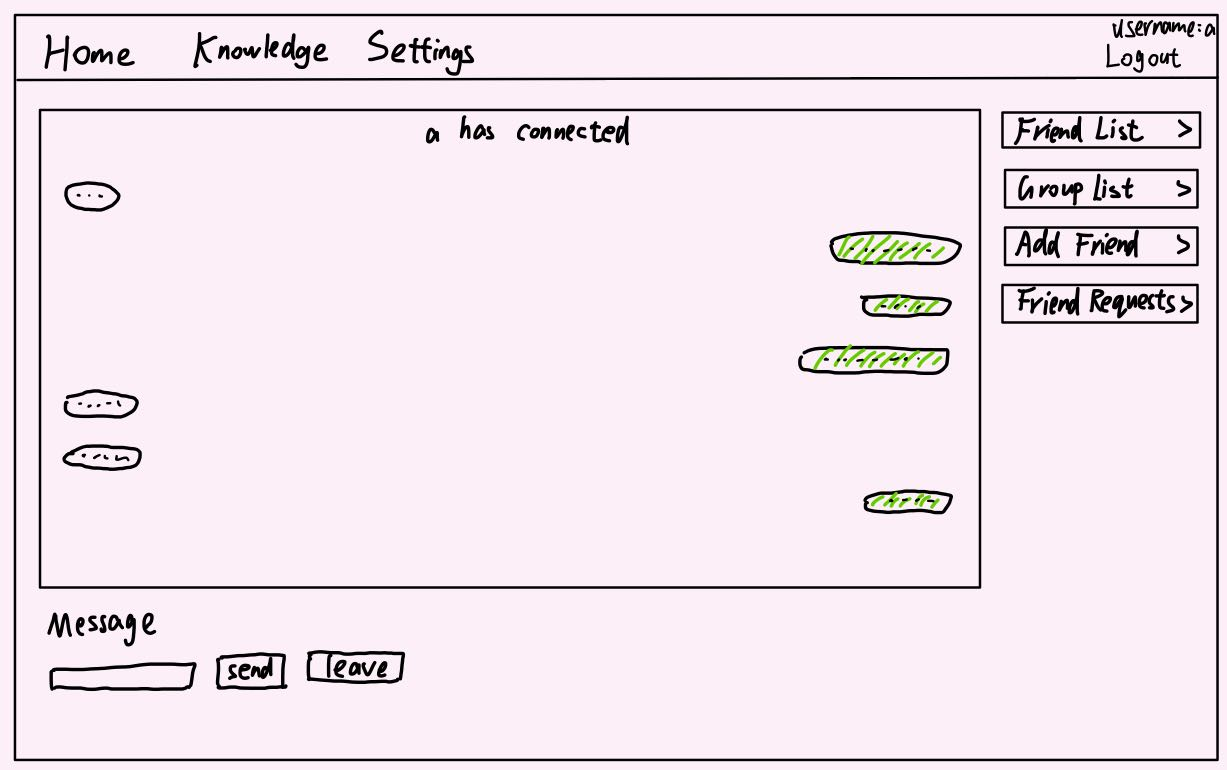
\includegraphics[width=0.8\textwidth]{graphs/message_page.jpg}
        \caption{Message Page}
        \label{Message Page}
    \end{figure}

    \begin{figure}[H]
        \centering
        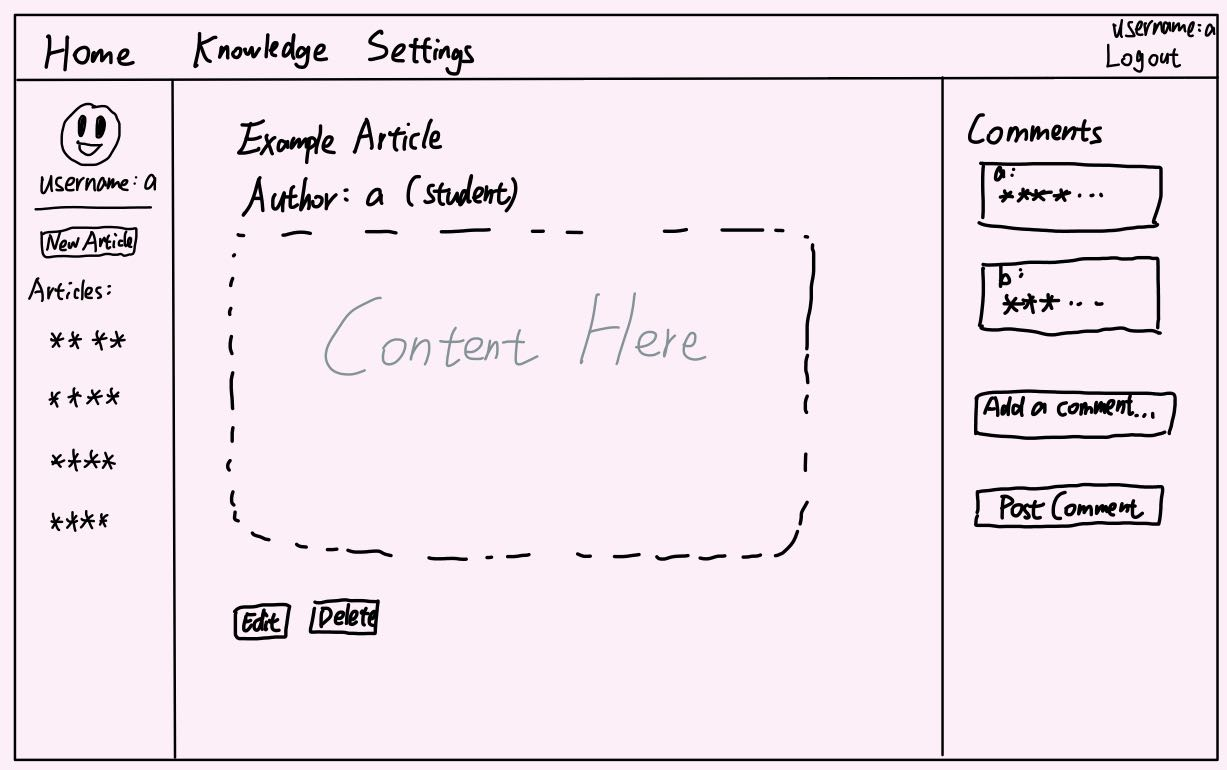
\includegraphics[width=0.8\textwidth]{graphs/knowledge_page.jpg}
        \caption{Knowledge Page}
        \label{Knowledge Page}
    \end{figure}

    \begin{figure}[H]
        \centering
        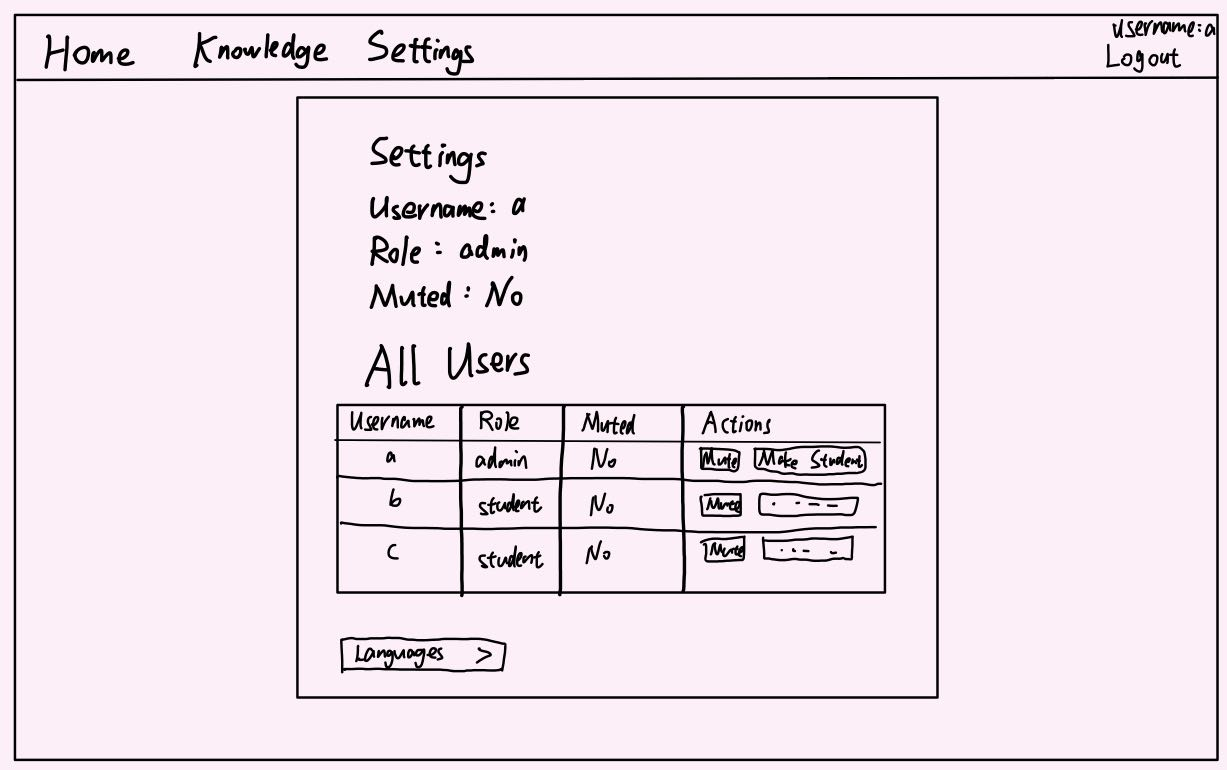
\includegraphics[width=0.8\textwidth]{graphs/setting_page.jpg}
        \caption{Setting Page}
        \label{Setting Page}
    \end{figure}



\subsection{Guerrilla Testing Report}

    \subsubsection*{Purpose} 
    \hspace{2em}The purpose of this testing is to evaluate the usability and user experience of the low-fidelity prototype, collect user feedback to improve the design, and identify necessary improvements in functionality and interface elements.

    \subsubsection*{Method}
        \begin{itemize}
            \item \textbf{Location}: Student accommodation Regiment 3090

            \item\textbf{Participants}:5 university students (mainly from the Computer Science major)

            \item \textbf{Tasks}
                \begin{enumerate}
                    \item Send a message to a friend on the messaging page.
                    \item Send a message to another friend.
                    \item Change the language preference in personal settings on the settings page.
                    \item Create and publish a new article on the knowledge repository page.
                    \item Comment on an article.
                \end{enumerate}

            \item \textbf{Tools} : Low-fidelity prototype (images)

        \end{itemize}

    \subsubsection*{Testing Procedure}
    \begin{itemize}
        \item\textbf{Steps}
            \begin{enumerate}
                \item Briefly introduce the purpose and process of the test.
                \item Have participants complete the tasks one by one while observing and recording their actions.
                \item Ask for participant feedback after each task.
            \end{enumerate}

        \item \textbf{Time}: Approximately 7 minutes per participant.
    \end{itemize}

    \subsubsection*{Raw Results}
        \begin{itemize}
            \item \textbf{Xu Jie | Computational Data Science}:\\
                The 'delete comment' button is way too small and hard to click. It would be much better if it were bigger. Also, the article list on the left is confusing. It should clearly show which articles are published by the user and which are not, maybe by adding some labels or filters.

            \item \textbf{James Zhao | Computer Science}: \\
                The different functions on the messaging page need clear dividers or background colors to make them stand out. The message box style should be more consistent for a smoother experience. And the action buttons should have prompts or descriptions so users know exactly what each one does.

            \item \textbf{Wenda Li | Computer Science}: \\
                The language settings button is kind of hard to spot. If there are a lot of users to manage on the admin page, scrolling all the way to the bottom to set the language is a hassle. For articles, maybe you can add an option to sort comments by time, like newest to oldest or vice versa?

            \item \textbf{Alex Zhou (Group Member)| Computer Science}: \\
                The interface makes it easy to tell what each function does.But in group chats, it’s hard to kown who sent each message. Maybe we should label the sender on each message?

            \item \textbf{Mingyuan Ba (Group Member)| Computer Science}: \\
                The page for articles looks clean, and the create/delete operations seem convenient. However, for an admin, it can be a trouble to browse through the entire list to find a user. It would be better to have a filter or search function.
        \end{itemize}



    \subsubsection*{Analysis}
        \begin{enumerate}
            \item \textbf{Messaging Page}
                \begin{itemize}
                    \item The boundaries between the four functional modules (e.g., sending messages, receiving messages, friend invitations, online status) are unclear and not obvious.
                    \item Group chat messages should display who sent the message
                    \item The style of the buttons should be more consistent.
                \end{itemize}

            \item \textbf{Knowledge Repository Page}
                \begin{itemize}
                    \item The article list on the left does not distinguish between all articles and those published by the user.
                    \item The "delete comment" button is too small and hard to click.
                \end{itemize}

            \item \textbf{Settings Page}
                \begin{itemize}
                    \item The behavior of actions is unclear, and users do not know how to perform specific operations.
                    \item Placing the language setting in a more prominent location would be preferable; placing it at the bottom of the settings page is not a good choice.
                \end{itemize}

        \end{enumerate}


    \subsubsection*{Conclusion}
        \begin{enumerate}
            \item \textbf{Main Findings} \\
            Overall interface design is good, but the messaging and settings pages need improvement, especially in the clarity of operations and interface. Multilingual settings are hard to find and need to be placed in a more prominent location.

            \item \textbf{Next Steps} \\
            Modify the layout of the messaging and settings pages based on the feedback, increase interface clarity and operation prompts, and prepare for the next round of testing.
        \end{enumerate}

\newpage

\section{Design-Evaluate 2}

\section{Appendix}

\subsection{User Investigation Survey Evidence}
\label{survey}
\textbf{Overview:}

\begin{figure}[H]
    \centering
    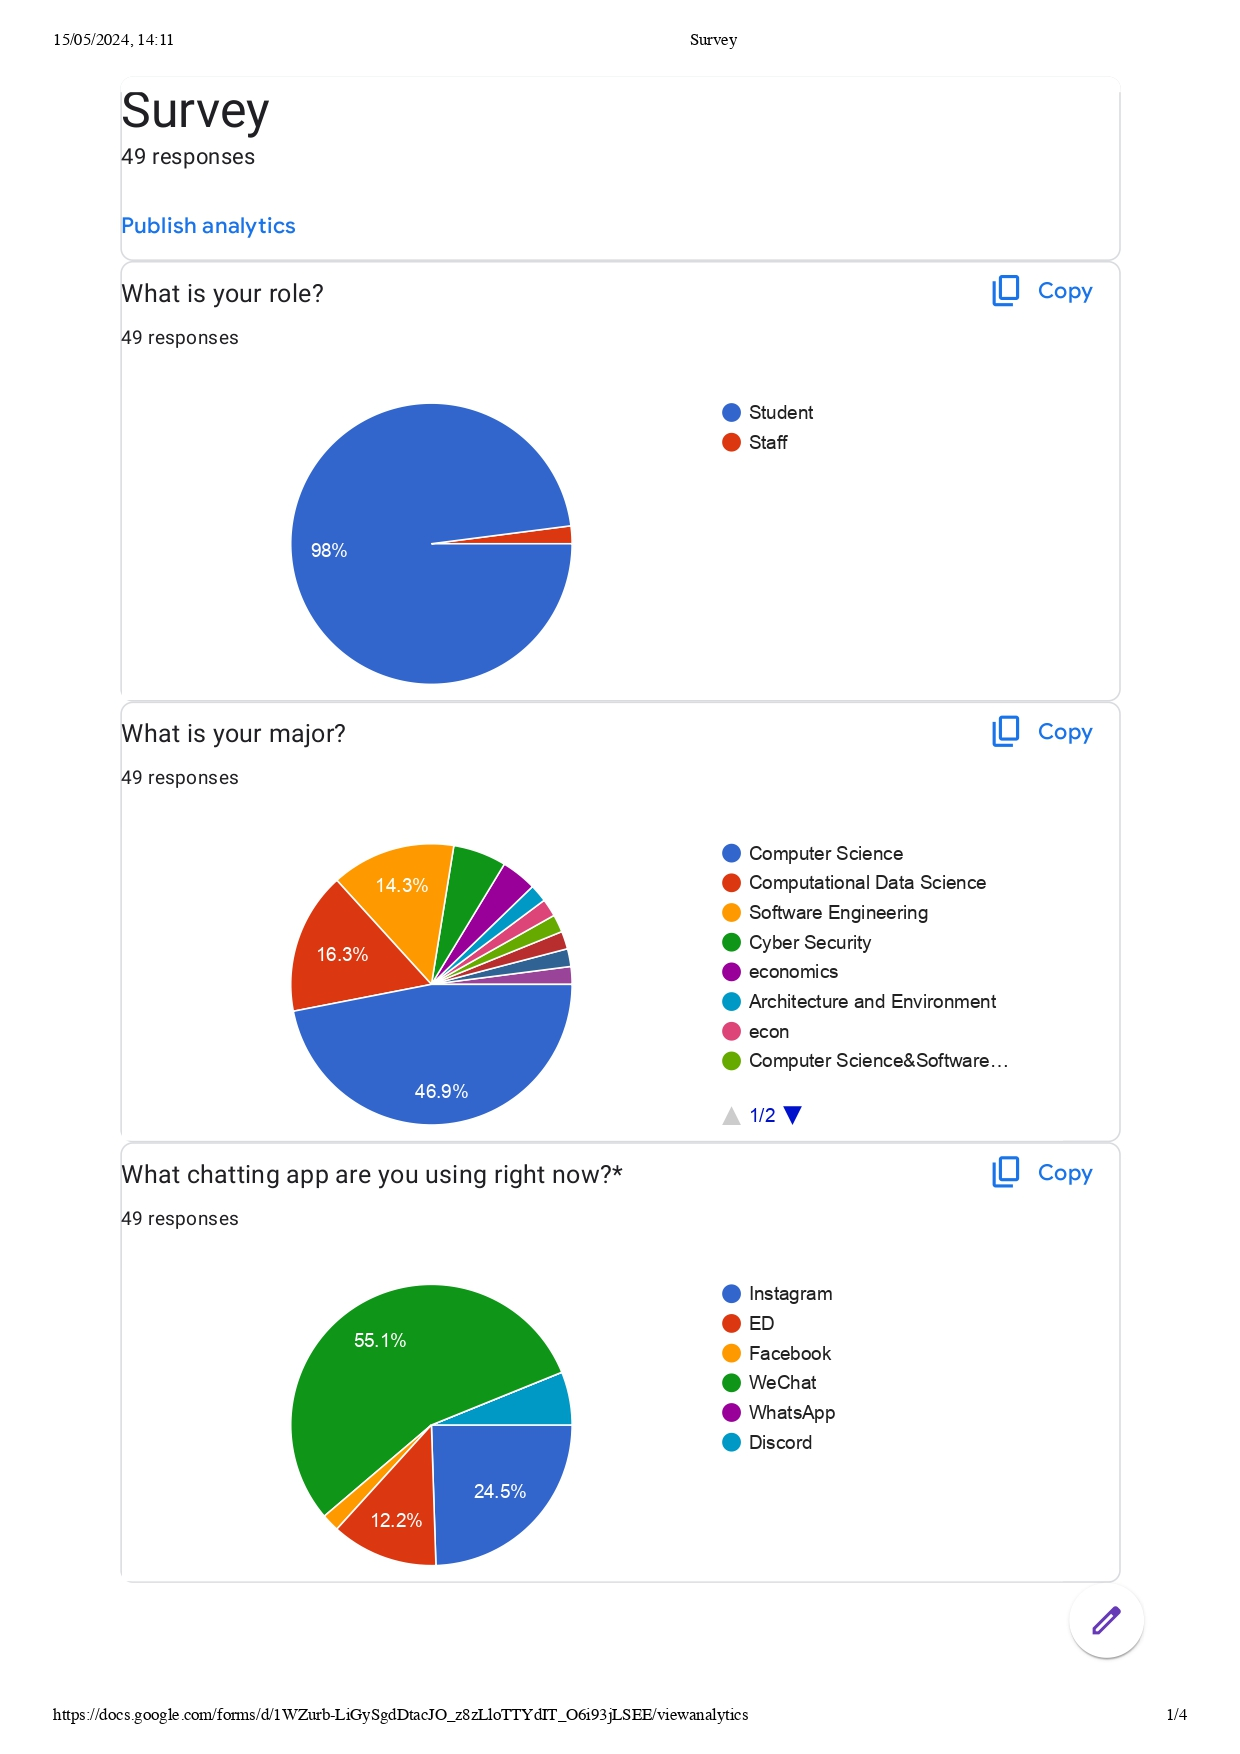
\includegraphics[width=0.9\textwidth]{graphs/Survey-summary_page-0001.jpg}
\end{figure}

\begin{figure}[H]
    \centering
    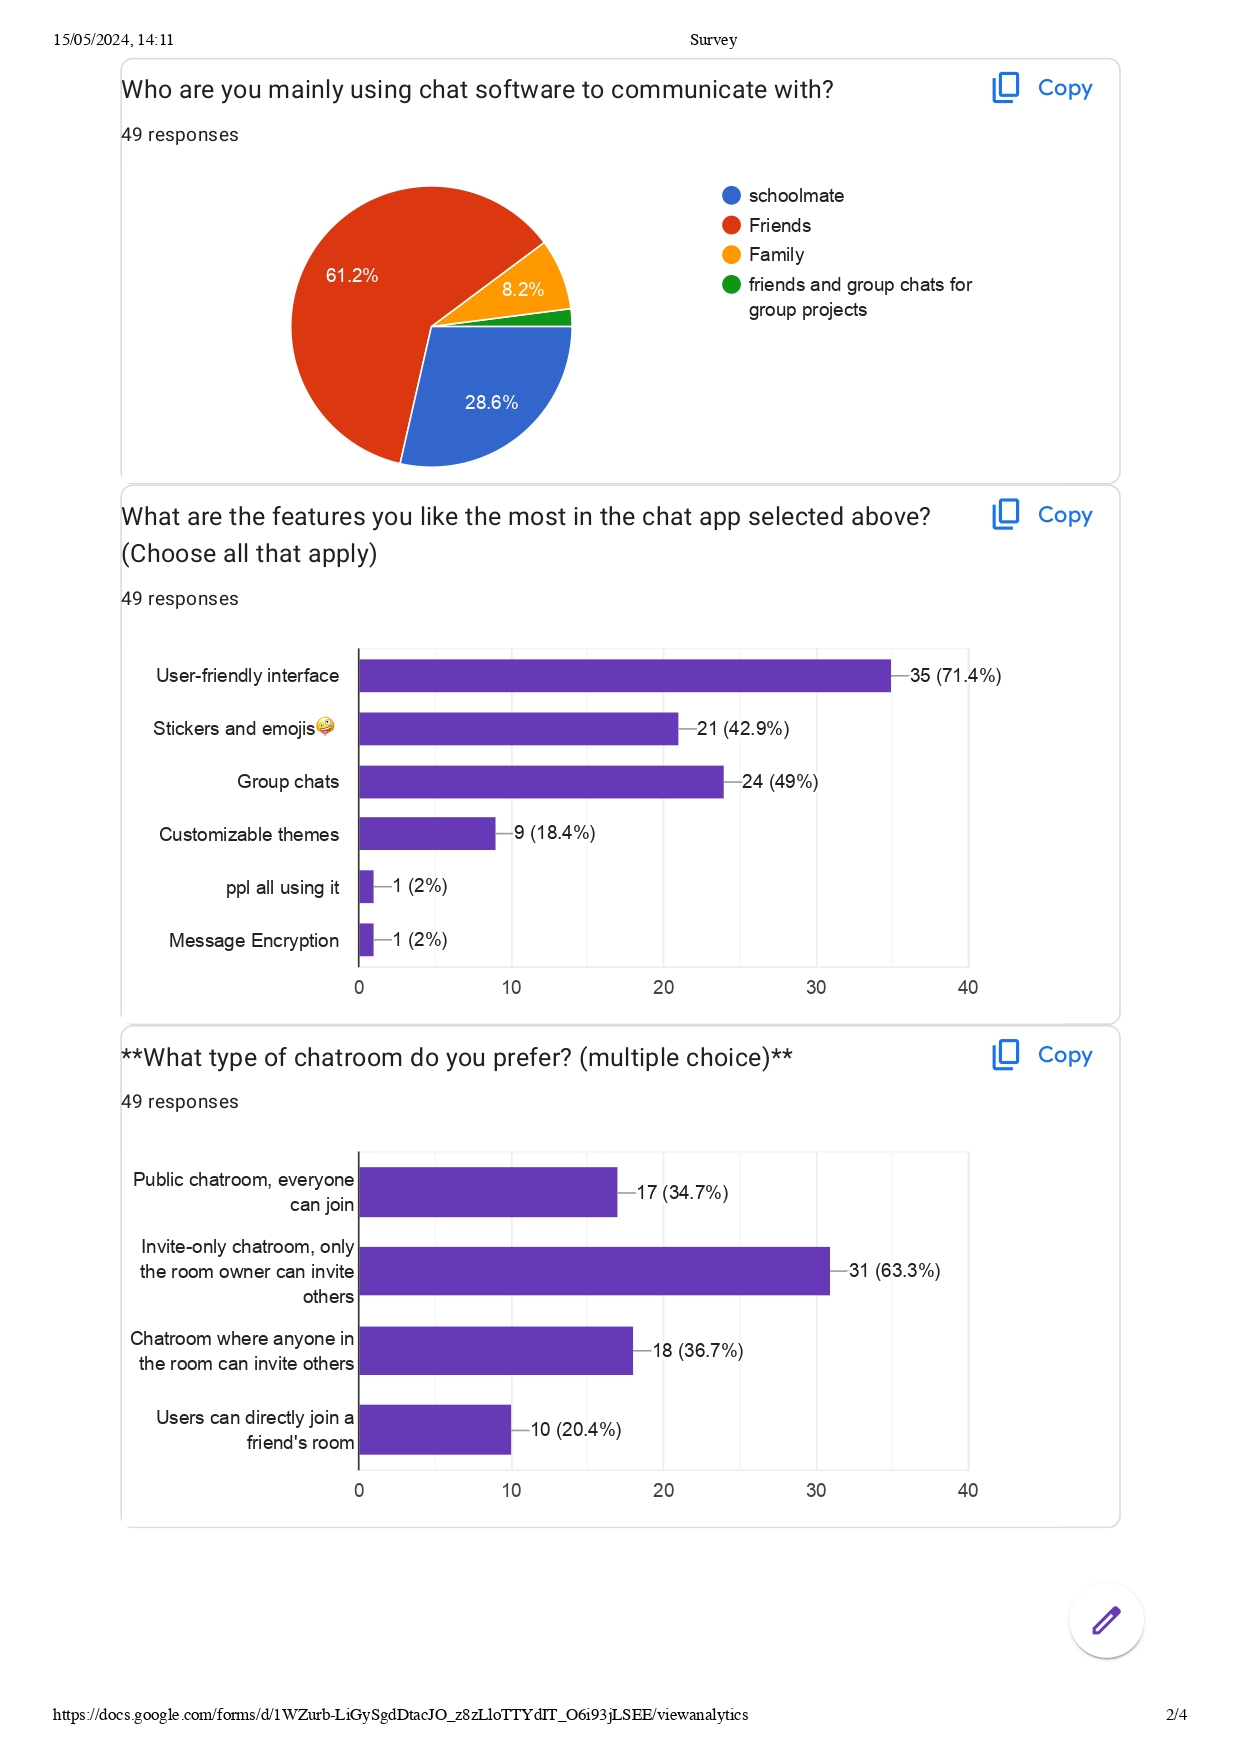
\includegraphics[width=0.9\textwidth]{graphs/Survey-summary_page-0002.jpg}
\end{figure}

\begin{figure}[H]
    \centering
    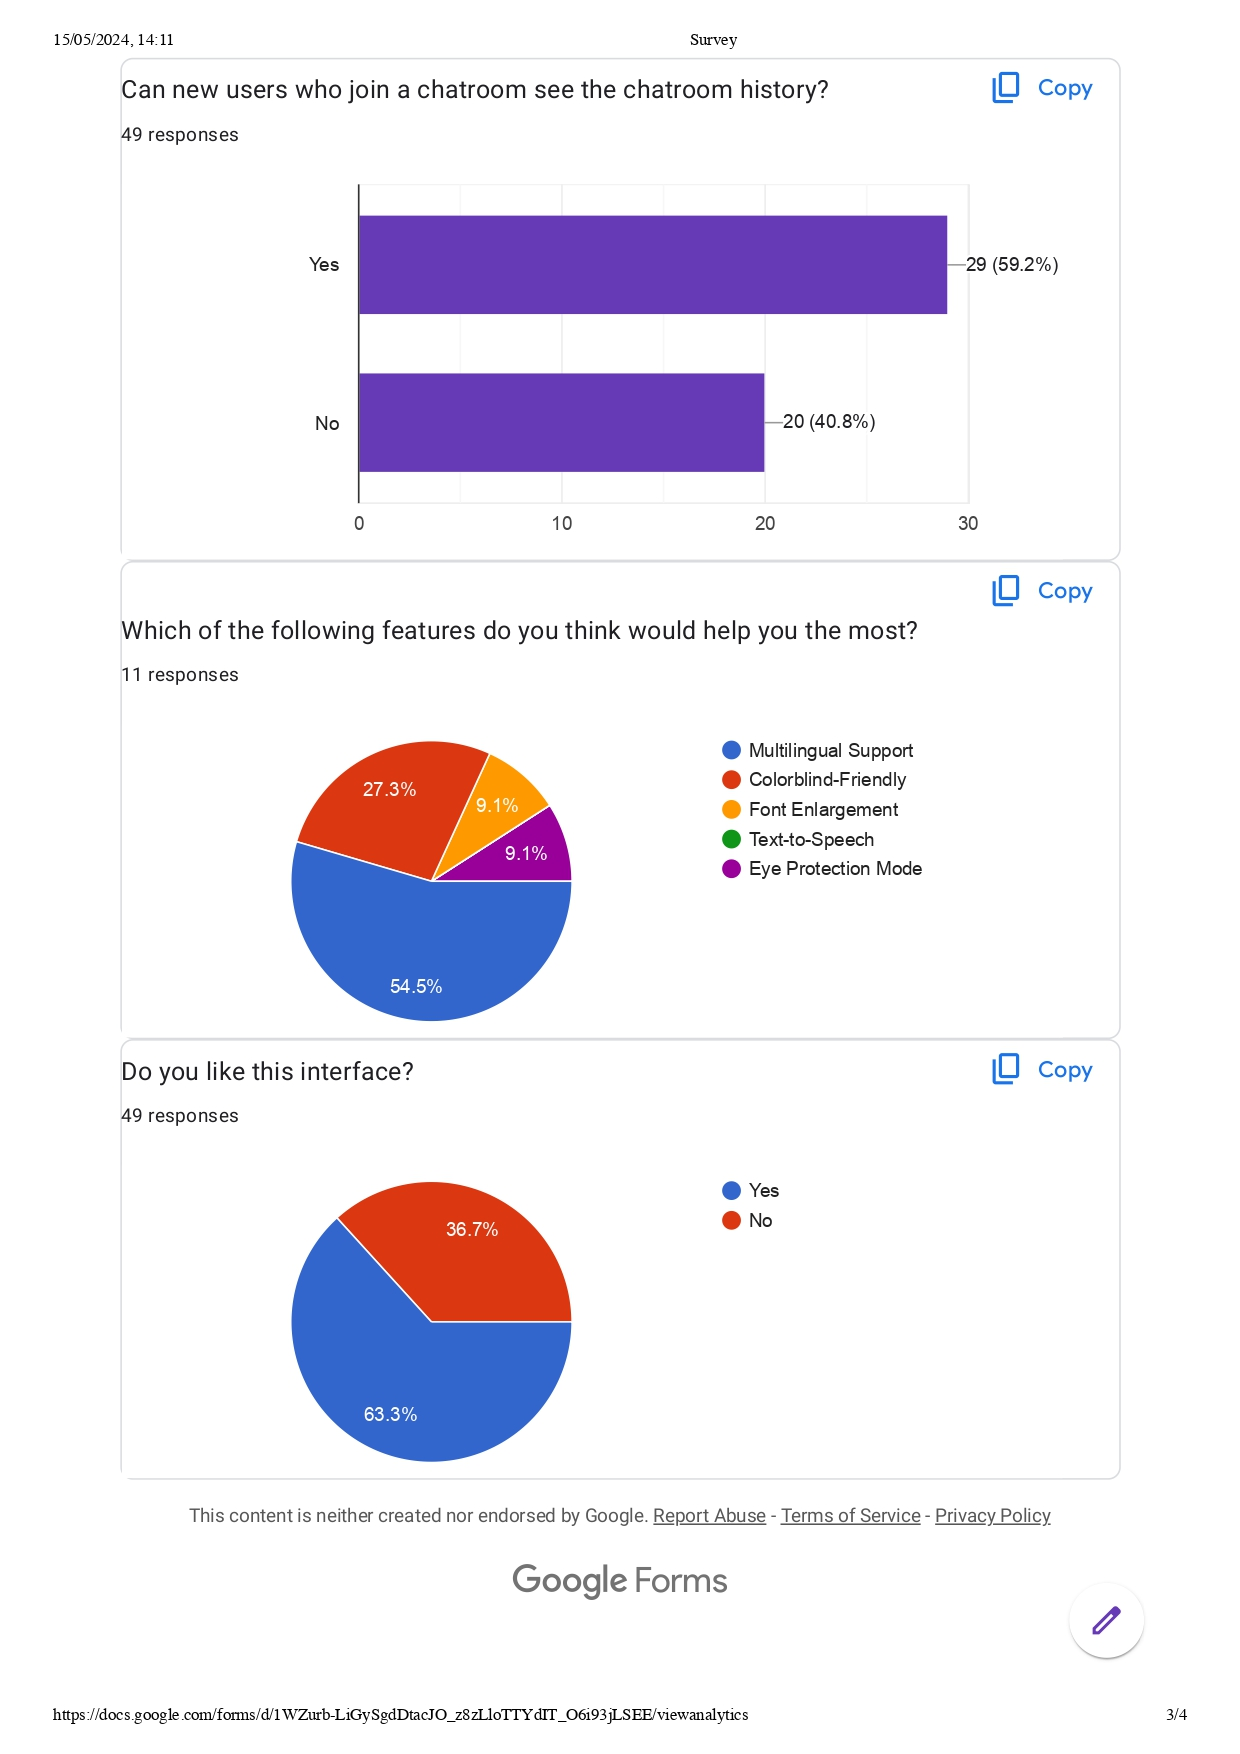
\includegraphics[width=0.9\textwidth]{graphs/Survey-summary_page-0003.jpg}
\end{figure}

\textbf{All Results}: /Evidence/Survey-all.pdf

\section{Contribution}

\bibliographystyle{unsrt}
\bibliography{reference} 
\end{document}
